\documentclass[letter,11pt]{article}
\usepackage{latexsym}
\usepackage{xcolor}
\usepackage{float}
\usepackage{amsthm}
\usepackage{esint}
\usepackage{amssymb}
\usepackage{wrapfig}
\usepackage{tabularx}
\usepackage{titlesec}
\usepackage{tikz}
\usepackage{geometry}
\usepackage{verbatim}
\usepackage{epstopdf}
\usepackage{enumitem}
\usepackage{fancyhdr}
\usepackage{pgfornament}
\usepackage{multicol}
\usepackage{systeme}
\usepackage{graphicx}
\usepackage{mathtools}
%\usepackage{cfr-lm}
\usepackage{booktabs}
\usepackage{svg}
\usepackage[T1]{fontenc}
\usetikzlibrary{trees}
\setlength{\multicolsep}{0pt} 
\pagestyle{fancy}
%\fancyhf{} % clear all header and footer fields
\fancyhead{}\fancyfoot{}
\fancyhead[R]{\textbf{\thepage}}
\fancyhead[L]{Aiden M. Rosenberg, MMXXIII A.D. }
\addtolength{\headwidth}{3cm}

\usepackage{pgfplots}
\pgfplotsset{compat=1.17}
\usepgfplotslibrary{fillbetween}

\usepackage{pst-plot}
\usepgfplotslibrary{polar}



\renewcommand{\headrulewidth}{1pt}
\renewcommand{\footrulewidth}{0pt}
\geometry{left=1.5cm, top=2.5cm, right=1.5cm, bottom=2cm}

%\usepackage{draftwatermark}	
%\SetWatermarkColor[gray]{0.9}
%\SetWatermarkText{Private}
%\SetWatermarkScale{3}

\usepackage[most]{tcolorbox}
\tcbset{
	frame code={}
	center title,
	left=0pt,
	right=0pt,
	top=0pt,
	bottom=0pt,
	colback=gray!20,
	colframe=white,
	width=\dimexpr\textwidth\relax,
	enlarge left by=-2mm,
	boxsep=4pt,
	arc=0pt,outer arc=0pt,
}


\raggedright
\setlength{\tabcolsep}{0in}

% Sections formatting
\titleformat{\section}{
  \vspace{-4pt}\scshape\raggedright\large
}{}{0em}{}[\color{black}\titlerule \vspace{-7pt}]

\titleformat{\subsection}[block]
  { \vspace{4pt}\bfseries\centering}
  {}{0em}{}

\begin{document}

\thispagestyle{empty}

\fontfamily{cmr}\selectfont
%----------HEADING-----------------

\parbox{2.35cm}{%
	\includesvg[width=2.3cm]{logo.svg}
}
\parbox{0.3cm}{\hspace{0.3cm}}
\parbox{\dimexpr\linewidth-5cm\relax}{
	\setlength{\tabcolsep}{0.5em}
	\def\arraystretch{1.25}
	\begin{tabular}{@{}llll@{}}
		\toprule
		\multicolumn{4}{c}
		{\hspace{-0.5em}\textbf{Assignment}: Worksheet \#8 (16.5)} \\ \midrule
		\textbf{Name:}   & D. Aiden M. Rosenberg & \textbf{Professor:} & Dr. Alan v. Herrmann Ph.D \\
		\textbf{Course:} & Calculus III          & \textbf{Date:}      & October 18th, 2023 A.D.   \\ \bottomrule
	\end{tabular} }
\vspace{1cm}

\section*{Section 16.5}

\subsection{Question \#1}
The integral $\displaystyle \int_{0}^{2\pi}\int_{0}^{2}\int_{0}^{2-2\sin\theta} r \, dz \, dr\, d\theta$
gives the volume of a solid. Sketch a well-labeled graph of the solid.
\begin{figure}[h]
    \centering
    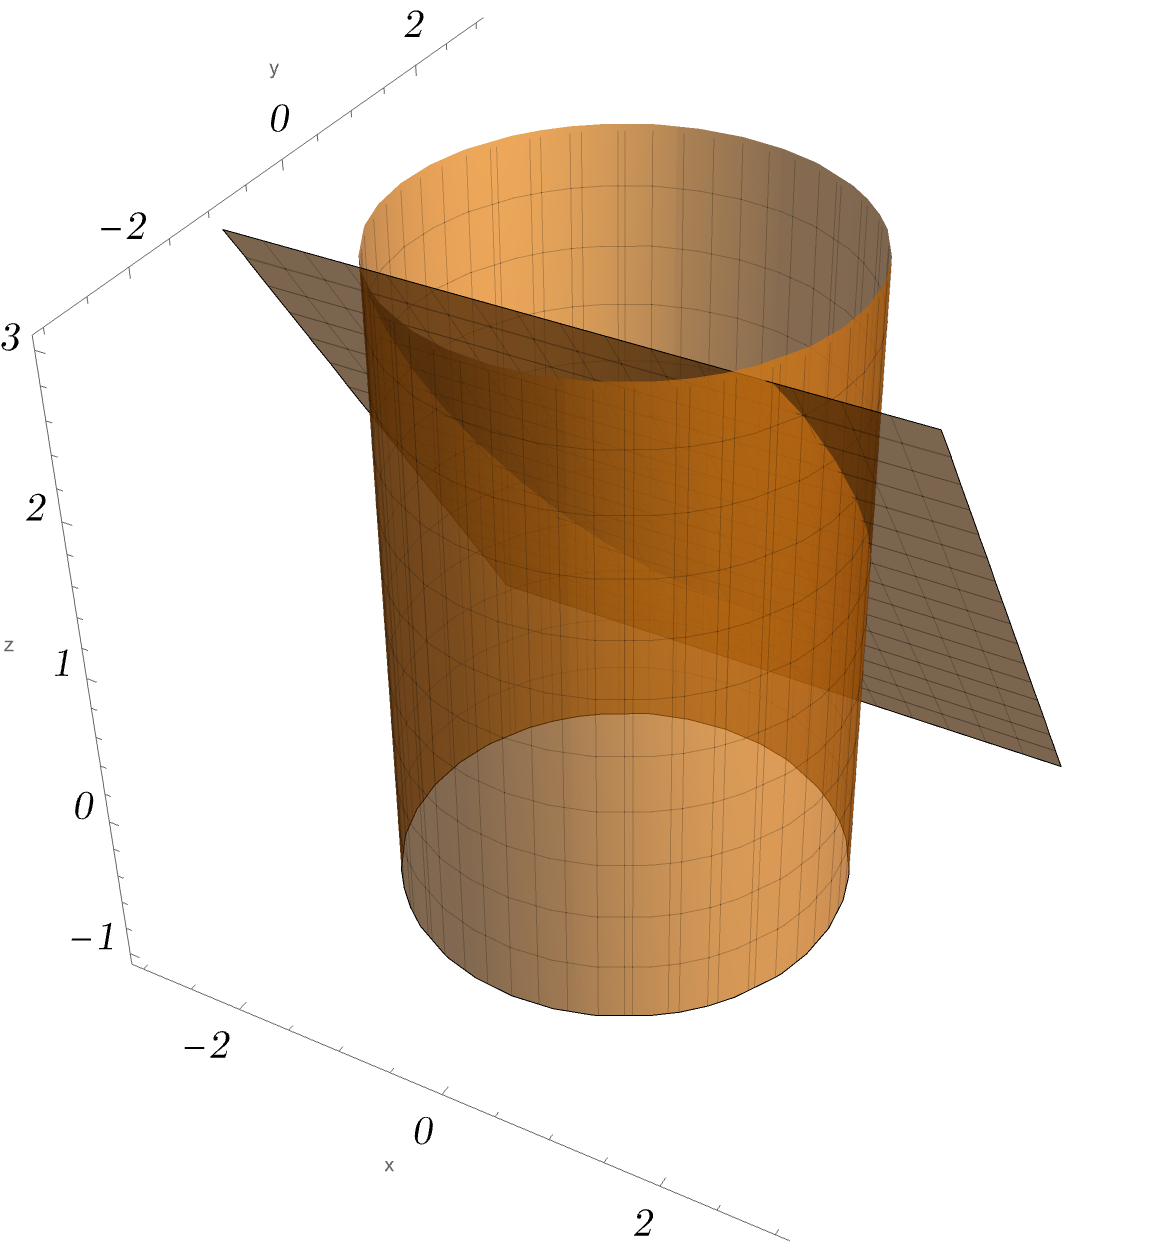
\includegraphics[width = 2in]{MyGraph.png}
    \caption{Graph of $4=x^2+y^2$ and $z=2-y$}
    \label{fig:enter-label}
\end{figure}
\subsection{Question \#2}
\begin{enumerate}[label = \roman*.]
    \item \underline{Set-up} a \textit{double integral} in polar coordinates to find the volume of the solid bounded above by $z = 10 -4x^2-4y^2$ and below by $z=4-x^2-y^2$.
    \begin{enumerate}
        \item $10-4x^2-4y^2 = 4-x^2-y^2 \Longrightarrow 2=x^2+y^2 \Longrightarrow r= \sqrt{2}$
    \end{enumerate}
    $$\boxed{\int_{0}^{2\pi}\int_{0}^{\sqrt{2}}\left(4-r^{2}\right) r\, dr\, d\theta}$$
    \item \underline{Set-up} a \textit{triple integral} in cylindrical coordinates to find the volume of the solid  above by $z = 10 -4x^2-4y^2$ and below by $z=4-x^2-y^2$.
    $$\boxed{\int_{0}^{2\pi}\int_{0}^{\sqrt{2}}\int_{4-r^{2}}^{10-4r^{2}}r \, dz\, dr \, d\theta }$$
\end{enumerate}
\newpage
\subsection{Question \#3}
Consider $\displaystyle \iiint_{E} \frac{1}{\sqrt{x^2+y^2+z^2}} \, dV$ where $E$ is bounded above by $x^2+y^2+z^2=4$ and and bounded below
by $z=\sqrt{3(x^2+y^2)}$. \underline{Set-up} the triple integral using:
\begin{enumerate}[label = \roman*.]
    \item Cartesian coordinates.
    $$\boxed{\int_{-1}^{1}\int_{-\sqrt{1-x^{2}}}^{\sqrt{1-x^{2}}}\int_{\sqrt{3}\sqrt{x^{2}+y^{2}}}^{\sqrt{4-x^{2}-y^{2}}}\left(\frac{1}{\sqrt{x^{2}+y^{2}+z^{2}}}\right) \, dz \, dy\, dx}$$
    \item Cylindrical coordinates.
    $$\boxed{\int_{0}^{2\pi}\int_{0}^{1}\int_{\sqrt{3}r}^{\sqrt{4-r^{2}}}\left(\frac{1}{\sqrt{r^{2}+z^{2}}}\right) \,dz\, r\, dr\, d\theta}$$
    \item Spherical coordinates. 
    \begin{enumerate}
        \item $\rho^2 = 4 \Longrightarrow \rho = 2$
        \item $\rho= \sqrt{3} \sqrt{x^2+y^2} \Longrightarrow \rho= \sqrt{3} \sqrt{p^2\sin^2\phi\cos^2\theta+p^2\sin^2\phi\sin^2\theta} \Longrightarrow \frac{1}{\sqrt{3}} = \sin\phi \Longrightarrow \phi = \frac{\pi}{6}$
    \end{enumerate}
    \begin{align*}
		&= \int_{0}^{2\pi}\int_{0}^{\frac{\pi}{6}}\int_{0}^{2} \frac{\rho^2\sin\phi}{\sqrt{\rho^2}} \, d\rho\, d\phi\, d\theta\\
        &= \int_{0}^{2\pi}\int_{0}^{\frac{\pi}{6}}\int_{0}^{2}\rho \sin\phi \, d\rho\, d\phi\, d\theta\\
        &= \int_{0}^{2\pi}\int_{0}^{\frac{\pi}{6}}\sin\phi \left[\frac{\rho^2}{2}\right]_{0}^{2}\, d\phi\, d\theta\\
        &= \int_{0}^{2\pi}\int_{0}^{\frac{\pi}{6}}2\sin\phi \,  d\phi\, d\theta\\
        &= \int_{0}^{2\pi}\left[-2\cos\phi\right]_{0}^{\frac{\pi}{6}}\, d\theta\\
        &= \int_{0}^{2\pi}\left(2-\sqrt{3}\right)\ d\theta\\
        &= \left[\left(2 - \sqrt{3}\right)\theta \right]_{0}^{2\pi}\\
        &= \boxed{2\pi\left(2 - \sqrt{3}\right)}
        \end{align*}
\end{enumerate}
\newpage
\subsection{Question \#4}
Evaluate $\displaystyle \iiint_{W} \left(x^2+y^2\right) \, dV$ where $W$ is the solid above $z=0$, inside $x^2+y^2=4$, and below $z=\sqrt{x^2+y^2}$.
\begin{enumerate}
    \item The solid lies above \(z = 0\), so the lower limit of integration for \(z\) is 0.
    \item The solid is inside \(x^2 + y^2 \leq 4\), which, in cylindrical coordinates, corresponds to \(0 \leq r \leq 2\).
    \item The solid is below \(z = \sqrt{x^2 + y^2}\), which, in cylindrical coordinates, is \(z \leq r\).
    
\begin{align*}
		&= \int_0^{2\pi} \int_0^2 \int_0^r (r^2) \, r \, dz \, dr \, d\theta\\
		&= \int_0^{2\pi} \int_0^2 \int_0^r (r^3) \, \, dz \, dr \, d\theta\\
		&= \int_{0}^{2\pi}\int_{0}^{2} \left[r^3 z\right]_{0}^r \, dr \, d\theta\\
		&= \int_{0}^{2\pi}\int_{0}^{2} r^4 \, dr \, d\theta\\
		&= \int_{0}^{2\pi} \left[\frac{r^5}{5}\right]_{0}^{2} \, d\theta\\
		&= \int_{0}^{2\pi} \frac{32}{5} \, d\theta\\
		&= \boxed{\frac{64 \pi}{5} }
        \end{align*}


\end{enumerate}

\subsection{Question \#5}
Evaluate $\displaystyle \int_{-3}^{3} \int_{-\sqrt{9-x^2}}^{\sqrt{9-x^2}}\int_{0}^{\sqrt{9-x^2-y^2}} e^{-\left(x^2+y^2+z^2\right)^{3/2}} \, dV$.
\begin{enumerate}
    \item Let $u = -\rho^3 \Longrightarrow du = -3\rho^2$
\end{enumerate}
\begin{align*}
    &= \int_{0}^{\pi}\int_{0}^{\pi}\int_{0}^{3}\left(e^{-\rho^{3}}\rho^{2}\sin\phi\right)\, d\rho\, d\phi\, d\theta\\
    &= \int_{0}^{\pi}\int_{0}^{\pi}\frac{-1}{3}\int_{0}^{-27}\left(e^{u}\sin\phi\right) \, du\, d\phi\, d\theta\\
    &= \frac{1}{3}\int_{0}^{\pi}\int_{0}^{\pi}\int_{-27}^{0}\left(e^{u}\sin\phi\right)\, du\, d\phi\, d\theta\\
    &= \frac{1}{3}\int_{0}^{\pi}\left(1-\frac{1}{e^{27}}\right) \left[-\cos(\phi)\right]_{0}^{\pi} \, d\theta\\
    &= \frac{2}{3}\left(1-\frac{1}{e^{27}}\right)\int_{0}^{\pi} \ d\theta \\
    &= \left[\frac{2}{3}\left(1-\frac{1}{e^{27}}\right) \theta \right]_{0}^{\pi}\\ &= \boxed{\frac{2}{3}\pi\left(1-\frac{1}{e^{27}}\right)}
\end{align*}
\end{document}
